\documentclass[11pt]{article}
\usepackage[a4paper,margin=25mm]{geometry}
\usepackage[T1]{fontenc}
\usepackage{lmodern,microtype,amsmath,amssymb,amsthm,mathtools}
\usepackage{booktabs,longtable,array,graphicx,xcolor}
\usepackage[breaklinks=true,colorlinks=true,linkcolor=blue!45!black,urlcolor=blue!50!black,citecolor=blue!50!black]{hyperref}
\hypersetup{pdftitle={Periodic obstructions to small-extrapolation Chambolle-Pock},
 pdfauthor={Dev D. Goyal},
 pdfsubject={Fully autonomous agentic research},
 pdfkeywords={Chambolle-Pock, PDHG, periodic orbits, Lean 4, convex optimization}}
\usepackage{enumitem,fancyhdr}
\setlist{itemsep=3pt,topsep=5pt,leftmargin=18pt}
\setlength{\parskip}{5pt}
\setlength{\parindent}{0pt}
\setlength{\emergencystretch}{2em}
\pagestyle{fancy}
\fancyhf{}
\fancyhead[L]{\small Periodic obstructions for Chambolle--Pock}
\fancyhead[R]{\small Dev D. Goyal}
\fancyfoot[C]{\thepage}
\setlength{\headheight}{14pt}
\newtheorem{theorem}{Theorem}[section]
\newtheorem{lemma}[theorem]{Lemma}
\newtheorem{proposition}[theorem]{Proposition}
\theoremstyle{remark}\newtheorem{remark}[theorem]{Remark}
\newcommand{\R}{\mathbb R}
\newcommand{\C}{\mathbb C}
\newcommand{\N}{\mathbb N}
\newcommand{\prox}{\operatorname{prox}}
\newcommand{\conv}{\operatorname{conv}}
\newcommand{\ip}[2]{\langle #1,#2\rangle}
\newcommand{\norm}[1]{\lVert #1\rVert}
\newcommand{\ind}{\iota}
\newcommand{\boundary}{K_3}
\newcommand{\replaystatus}{A fresh replay on 30 October 2026, compiling all 21 modules from source against a Mathlib checkout built at the pinned revision, passed with all 45 axiom audits; its record is in \texttt{verification/}.}
\newcommand{\leanname}[1]{\begingroup\small\urlstyle{tt}\nolinkurl{#1}\endgroup}
\title{\vspace{-15mm}\textbf{Periodic obstructions to small-extrapolation\\Chambolle--Pock}\\[5pt]
\large An exact three-cycle threshold, robust seven-cycles,\\and a four-dimensional Fourier construction}
\author{Dev D. Goyal}
\date{30 October 2026}
\begin{document}
\maketitle
\thispagestyle{empty}

\section*{Research process and AI disclosure}
This is fully autonomous agentic research. Dev D. Goyal is responsible for publication. No expert validation or external peer review is claimed, and the novelty assessment is provisional.

The research, the constructions and certificates, the Lean formalization and an earlier report were produced by autonomous AI research agents in an earlier session whose records do not name the model or system used.

Opus 5.5 by Anthropic used with Claude Code assessed that package for this release. It coordinated an independent AI referee check, which recomputed the three-cycle identity and the seven-cycle certificate with new exact-arithmetic code and simulated the Fourier family. It ran the fresh Lean replay described in Section~\ref{sec:verification} and rewrote this manuscript, adding the scope and limitations in Section~\ref{sec:limits}. AI referee checks are not human peer review. Lean verification establishes only the formal statements listed in Section~\ref{sec:verification}.

\begin{abstract}
We investigate necessary restrictions on the convergence region of the unchanged Chambolle--Pock method at small positive extrapolation. A dimension-independent sum-of-squares identity gives the exact universal step-product threshold for a nonconstant three-cycle, and compact triangles attain that threshold. An independent pair of integer-coordinate polytopes in $\R^4$ yields a seven-cycle on a full parameter rectangle near step product $5/2$, below the three-cycle threshold. Every sufficiently close initial state is captured by that seven-cycle after one update. A mixed-frequency construction gives a further family: for every fixed step product greater than $2$, suitable compact polytopes in $\R^4$ cycle for all sufficiently small positive extrapolation. The constructions have a saddle point and use actual global proximal minimizers. We give mathematical proofs, exact certificates and Lean 4 proofs. These are necessary obstructions, not a determination of the full convergence region, and the obstructing extrapolation intervals are very small. No matching antecedent was located in the inspected literature; priority is provisional.
\end{abstract}
\tableofcontents
\newpage

\section{The question and the precise algorithm}

Let $E,F$ be real Hilbert spaces, $L:E\to F$ a bounded linear operator, and $f,h$ proper lower semicontinuous convex functions. Consider the saddle problem
\begin{equation}\label{eq:saddle}
  \min_{x\in E}\max_{y\in F}\; f(x)+\ip{Lx}{y}-h(y).
\end{equation}
The unchanged primal-first Chambolle--Pock iteration is
\begin{equation}\label{eq:cp}
\begin{aligned}
 x^{k+1}&=\prox_{\tau f}(x^k-\tau L^*y^k),\\
 y^{k+1}&=\prox_{\sigma h}\bigl(y^k+\sigma L((1+\theta)x^{k+1}-\theta x^k)\bigr).
\end{aligned}
\end{equation}
Here $\tau,\sigma>0$, and the parameter of interest is
\[
 \kappa=\tau\sigma\norm{L}^2.
\]
There is no additional relaxation or correction of the pair $(x^{k+1},y^{k+1})$. This point matters when comparing results for related splitting algorithms.

Banert, Upadhyaya and Giselsson prove weak convergence for $\theta>1/2$ and $\kappa<4/(1+2\theta)$, and their scalar bilinear example fails at and above that bound \cite{BUG}. Upadhyaya's 2026 preprint, in the version of 20 August 2026, establishes weak convergence for $0<\theta\le1/2$ under the explicit sufficient condition
\begin{equation}\label{eq:known}
 \kappa< B_{\rm suf}(\theta):=
 \frac{4\theta(2-\theta)}{1-2\theta+9\theta^2-4\theta^3}.
\end{equation}
Its conclusion leaves improvement of the small-$\theta$ region open \cite{U26}. Numerical Lyapunov feasibility regions and larger-memory certificates provide additional information, but infeasibility of a selected certificate does not prove failure of the algorithm \cite{AutoTight,AutoLyap}.

The present investigation addresses the complementary necessary-condition question: how far can a guarantee over \emph{all} convex problems extend? Its strongest candidate theorem is the fixed-dimension family approaching step product $2$ as $\theta\downarrow0$. The exact three-cycle classification supplies a second, structural conclusion; the seven-cycle supplies a simple rational example with an open basin of nonconvergence.

\subsection{Results at a glance}

Define
\begin{align}
 \Delta(\kappa,\theta)&=\kappa^2(1+\theta)^2-2\kappa(1+3\theta)-3,\label{eq:delta}\\
 \boundary(\theta)&=
 \frac{1+3\theta+\sqrt{(1+3\theta)^2+3(1+\theta)^2}}{(1+\theta)^2}.
 \label{eq:kthree}
\end{align}

\begin{theorem}[Universal three-cycle boundary]\label{thm:three}
For $\theta\ge0$, any nonconstant three-periodic orbit of actual convex proximal updates \eqref{eq:cp} satisfies
\[
 \Delta(\tau\sigma\norm{L}^2,\theta)\ge0,
 \quad\text{equivalently}\quad \tau\sigma\norm{L}^2\ge\boundary(\theta).
\]
Conversely, for every $\kappa>0$ and $\theta\ge0$ satisfying this inequality, there are compact convex triangles, with a saddle point, whose projection version of \eqref{eq:cp} has a nonconstant three-cycle at $L=I$, $\tau=1$, $\sigma=\kappa$.
\end{theorem}

\begin{theorem}[Robust rational seven-cycle]\label{thm:seven}
There are fixed compact convex polytopes $C,D\subset\R^4$, given explicitly in Section~\ref{sec:seven}, such that $(0,0)$ is a saddle of \eqref{eq:saddle} for $f=\ind_C$, $h=\ind_D$, $L=I$. For every
\begin{equation}\label{eq:rectangle}
 \frac{2499}{1000}\le\kappa\le\frac{2501}{1000},
 \qquad 0\le\theta\le\frac1{400},
\end{equation}
the update with $\tau=1$, $\sigma=\kappa$ has a nonconstant seven-periodic orbit. In a neighborhood of every state on the orbit, all initial states agree with that orbit from their first update onward. In particular, an open set of initial states fails to converge. Throughout \eqref{eq:rectangle},
\[
 \kappa<\boundary(\theta)\quad\text{and}\quad
 \kappa<\frac4{1+2\theta}.
\]
\end{theorem}

\begin{theorem}[Four-dimensional obstruction above two]\label{thm:asymptotic}
For every fixed $\kappa>2$, there are compact convex polytopes $C,D\subset\R^4$, both containing zero, and $\varepsilon>0$ such that the same pair $C,D$ produces a nonconstant periodic orbit of \eqref{eq:cp} for every $0\le\theta\le\varepsilon$, with $f=\ind_C$, $h=\ind_D$, $L=I$, $\tau=1$, and $\sigma=\kappa$. These actual iterates do not converge, despite the saddle $(0,0)$.
\end{theorem}

For $2<\kappa<4$, one can decrease $\varepsilon$ so that every positive $\theta$ in the resulting interval also satisfies $\kappa<4/(1+2\theta)$. This is a nonlinear obstruction inside the stability range of the quadratic eigenmodes analyzed in Section~\ref{sec:quad}. No matching sufficiency theorem below $2$ is asserted. Nor does Theorem~\ref{thm:asymptotic} assert attraction; its primal normal vectors vanish, unlike the strict seven-cycle certificate.

\begin{figure}[htbp]
\centering
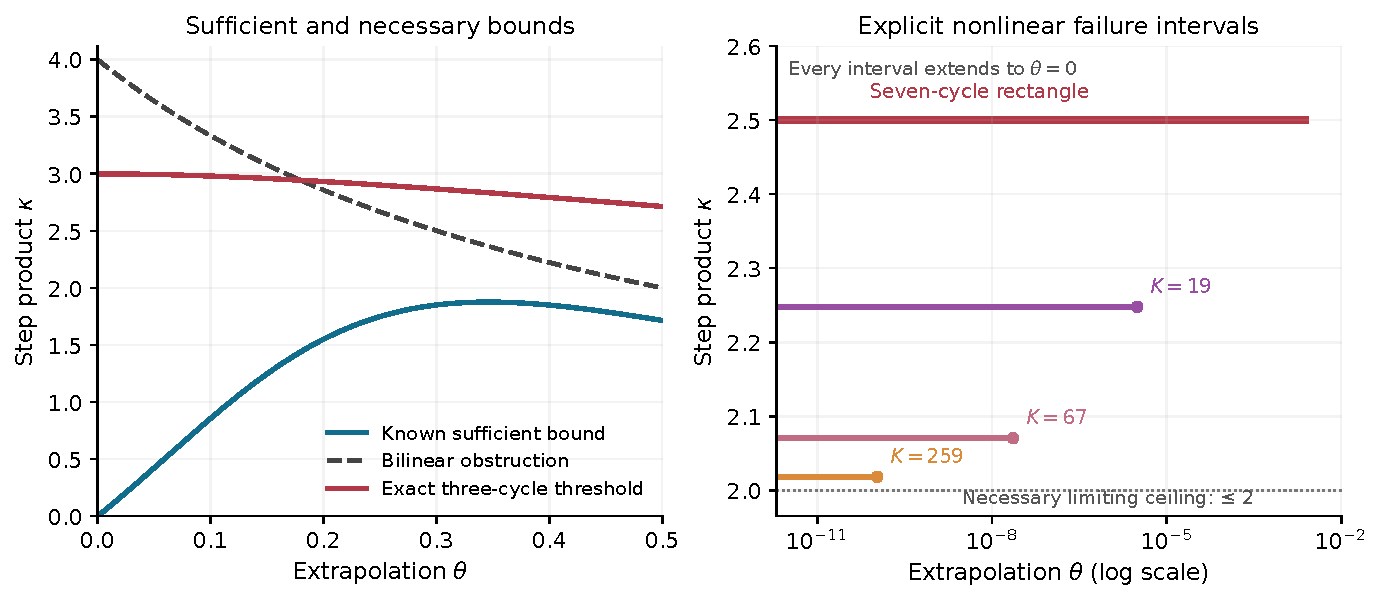
\includegraphics[width=\textwidth]{figures/parameter_bounds.pdf}
\caption{Left: the published explicit sufficient bound \eqref{eq:known}, the bilinear necessary obstruction, and the exact three-cycle threshold. Right: explicit instances of the proved Fourier family with $\kappa=2+3\sin(\pi/(2K))$, together with the seven-cycle rectangle. Every horizontal interval continues to zero; the logarithmic display omits its left endpoint. The limiting ceiling is a necessary restriction, not a sharp convergence threshold. Curves and endpoints are numerical displays of exact formulas; no plot is used as a proof.}
\label{fig:bounds}
\end{figure}

\section{Actual proximal minimization and finite certificates}\label{sec:prox}

To model extended-valued objectives without hiding their domains, let $C\subset E$ be convex and let $f:C\to\R$ be convex. Extend $f$ arbitrarily to a real function on $E$; its values outside $C$ are ignored. The assertion that $x$ is a proximal minimizer at center $c$ means
\begin{equation}\label{eq:isprox}
 x\in C,\qquad
 f(x)+\tfrac12\norm{x-c}^2\le f(z)+\tfrac12\norm{z-c}^2
 \quad\text{for all }z\in C.
\end{equation}
It is equivalent to the supporting inequality
\begin{equation}\label{eq:support}
 f(x)+\ip{c-x}{z-x}\le f(z)\qquad(z\in C).
\end{equation}
For completeness, \eqref{eq:support} implies \eqref{eq:isprox} by expanding the square. Conversely, insert $x+t(z-x)$ into \eqref{eq:isprox}, use convexity, divide by $t>0$, and let $t\downarrow0$. The resulting supporting inequalities also prove uniqueness: applying them to two minimizers gives the squared distance between those minimizers at most zero. These statements are formalized, not assumed.

When $f=0$ on the convex hull of finitely many vertices $v_j$, the supporting inequality is equivalent to
\begin{equation}\label{eq:vertexcert}
 \ip{c-v_i}{v_j-v_i}\le0\quad\text{for every vertex }v_j.
\end{equation}
Linearity extends the inequalities to the entire convex hull. Compactness gives a global minimizer at every center, and uniqueness identifies it as the metric projection. Thus checking \eqref{eq:vertexcert} certifies the actual projection map, including its behavior under arbitrary repeated iteration.

If every inequality in \eqref{eq:vertexcert} is strict for $j\ne i$, continuity and finiteness give a neighborhood of $c$ with the same projected vertex $v_i$. Applying this argument to the two successive CP projection centers proves local constancy of the entire update near a strictly certified cycle state. This is the mechanism behind the exact one-step capture in Theorem~\ref{thm:seven}.

\section{The universal three-cycle certificate}

\subsection{Supporting sums and the sum-of-squares identity}

First normalize to $\tau=1$, dual step $\kappa$, and a contraction $L$, and write $a_i=Lx_i$. All indices in this section are interpreted modulo three. A three-cycle supplies support vectors
\[
 p_i=x_{i-1}-x_i-L^*y_{i-1},\qquad
 q_i=y_{i-1}-y_i+\kappa((1+\theta)a_i-\theta a_{i-1}).
\]
The convex inequalities at each point, tested against the next point, telescope. Therefore
\begin{align*}
 A&:=\sum_{i=0}^2\ip{x_{i-1}-x_i}{x_{i+1}-x_i}
       -\sum_{i=0}^2\ip{y_{i-1}}{a_{i+1}-a_i}\le0,\\
 B&:=\sum_{i=0}^2\ip{q_i}{y_{i+1}-y_i}\le0.
\end{align*}
Set
\[
 U=\sum_i\norm{x_i-x_{i+1}}^2,\qquad
 W=\sum_i\norm{a_i-a_{i+1}}^2,
\]
so $W\le U$, and define
\[
 Z_i=(y_i-y_{i+1})-\frac{\kappa(1+\theta)}2(a_i-a_{i+1})
           -\frac12(2a_{i-1}-a_i-a_{i+1}).
\]
The exact identity is
\begin{equation}\label{eq:sos}
\begin{aligned}
 \Delta(\kappa,\theta)U
   ={}&4\sum_i\norm{Z_i}^2-8B
       -4\bigl(3+\kappa(1+3\theta)\bigr)A\\
      &+\bigl(\kappa^2(1+\theta)^2+3\bigr)(U-W).
\end{aligned}
\end{equation}
It follows by expanding inner products and collecting coefficients. The Lean proof checks the expansion for arbitrary real inner-product spaces; it is not a numerical Gram-matrix certificate.

For $\kappa,\theta\ge0$, every term on the right of \eqref{eq:sos} is nonnegative. If the full state cycle is nonconstant then $U>0$: otherwise all $x_i$ agree, and the dual supporting sum reduces to $\frac12\sum_i\norm{y_i-y_{i+1}}^2$, which must vanish. Dividing by $U$ proves $\Delta\ge0$.

\subsection{Restoring the genuine steps and operator norm}

For $L\ne0$, let $r=\norm{L}$, replace $a_i$ by $Lx_i/r$, replace $y_i$ by $\tau r y_i$, and put $\kappa=\tau\sigma r^2$. The normalized primal supporting sum equals the original primal sum, while the normalized dual sum is the original dual sum multiplied by $(\tau r)^2$. The contraction estimate follows from $\norm{Lz}\le r\norm z$. Thus \eqref{eq:sos} applies with the exact product $\tau\sigma\norm L^2$.

When $L=0$, the two blocks are independent proximal iterations. Summing their three supporting inequalities forces each block's displacement energy to vanish. Consequently there is no nonconstant three-cycle. This case is included in the final formal necessity theorem; it is not excluded by an unstated nonzero-operator assumption.

Solving the quadratic inequality \eqref{eq:delta} for nonnegative $\kappa$ gives precisely \eqref{eq:kthree}. Both non-strict and strict root comparisons are formalized.

\subsection{Attainment by compact triangles}

In $\R^3$, put
\[
 x_0=(2,-1,-1),\quad x_1=(-1,2,-1),\quad x_2=(-1,-1,2),
\]
and, with cyclic indices, set
\[
 y_i=sx_i+b(x_{i-1}-x_{i+1}),\qquad
 C=\conv\{x_0,x_1,x_2\},\quad D=\conv\{y_0,y_1,y_2\}.
\]
The vertices lie in the zero-sum plane. The formal ambient space is $\R^3$; no unformalized reduction of dimension is needed for the theorem. Both vertex sums vanish, hence $0\in C\cap D$, and $(0,0)$ is a saddle for the restricted bilinear objective.

Writing $Q=s^2+3b^2$, the vertex normal conditions reduce to four scalar inequalities:
\begin{equation}\label{eq:triangleineqs}
\begin{gathered}
 b\ge\tfrac12,\qquad s+b\ge2,\\
 Q\le\kappa\bigl((1+\theta)s-(1+3\theta)b\bigr),\qquad
 2Q\le\kappa\bigl((1+2\theta)s+b\bigr).
\end{gathered}
\end{equation}
They certify
\[
 P_C(x_{i-1}-y_{i-1})=x_i,\qquad
 P_D\bigl(y_{i-1}+\kappa((1+\theta)x_i-\theta x_{i-1})\bigr)=y_i.
\]
Choose
\[
 b=\tfrac12,\qquad s=\tfrac12\kappa(1+\theta).
\]
The inequality $\Delta\ge0$ implies $\kappa(1+\theta)\ge3$, yielding the first two conditions. The third is exactly $\Delta\ge0$ after multiplication by four. The fourth follows from nonnegativity of $\kappa\theta(\kappa(1+\theta)-1)$. All four are checked symbolically in Lean. Since $x_0\ne x_1$, two constant subsequences of the actual iterates have different values, proving nonconvergence.

The fixed choice $s=3/2$, $b=1/2$, $\kappa=3$ works for every $\theta\ge0$. It is strictly below the bilinear boundary when $0<\theta<1/6$. More generally, exact algebra gives
\begin{equation}\label{eq:cross}
 \boundary(\theta)<\frac4{1+2\theta}
 \quad\Longleftrightarrow\quad
 44\theta^2+20\theta<5
 \quad\Longleftrightarrow\quad
 0\le\theta<\frac{4\sqrt5-5}{22}.
\end{equation}
The last endpoint is about $0.179285$. This improves a necessary obstruction over an interval, but cannot be used as a convergence boundary.

\section{The explicit seven-cycle and its open basin}\label{sec:seven}

Let $C=\conv\{X_i:0\le i<7\}$ and $D=\conv\{Y_i:0\le i<7\}$, where the rows below are the integer vectors actually used in Lean.

\begin{center}\small
\begin{tabular}{r|rrrr|rrrr}
\toprule
$i$&\multicolumn{4}{c|}{$X_i$}&\multicolumn{4}{c}{$Y_i$}\\
\midrule
0&768&0&7454&0&259&-896&9234&-7329\\
1&481&602&-1660&7266&861&-350&5097&10633\\
2&-170&749&-6714&-3234&812&455&-11500&2597\\
3&-695&336&4647&-5824&154&917&22&-11788\\
4&-695&-336&4647&5824&-623&693&11488&2646\\
5&-170&-749&-6714&3234&-931&-56&-5137&10612\\
6&481&-602&-1660&-7266&-532&-763&-9204&-7371\\
\bottomrule
\end{tabular}
\end{center}

For each $i$ modulo seven, the exact certificate is
\begin{align}
 &\ip{X_i-Y_i-X_{i+1}}{X_j-X_{i+1}}<0,
       &&j\ne i+1,\label{eq:sevenprimal}\\
 &\ip{Y_i+\kappa((1+\theta)X_{i+1}-\theta X_i)-Y_{i+1}}
        {Y_j-Y_{i+1}}<0,
       &&j\ne i+1.\label{eq:sevendual}
\end{align}
These hold throughout the closed rectangle \eqref{eq:rectangle}. The excluded diagonal cases have value zero, as required by a normal-cone inequality.

An independent standard-library Python audit checks the coordinates after division by $14{,}000$, using exact rational arithmetic. Its maximum off-diagonal primal value is $-429/2{,}800{,}000$. The maximum dual values at the four corners are:

\begin{center}
\begin{tabular}{ccc}
\toprule
$\kappa$ & $\theta$ & Maximum dual support value\\
\midrule
$2499/1000$&$0$&$-2622853/800000000$\\
$2499/1000$&$1/400$&$-96724819/320000000000$\\
$2501/1000$&$0$&$-1324939/400000000$\\
$2501/1000$&$1/400$&$-255773241/800000000000$\\
\bottomrule
\end{tabular}
\end{center}

There are 42 off-diagonal primal tests and 42 dual tests at each corner. Each dual expression is affine in either parameter while the other is fixed, so negativity at the corners suffices on the rectangle. The separate Lean proof establishes the inequalities directly for arbitrary real parameters with those bounds. Neither the rational checker nor a numerical solver is trusted by the Lean proof.

The two vertex sums are exactly zero, and $X_0\ne X_1$. Section~\ref{sec:prox} now identifies the actual CP update with cyclic advancement through these seven states and proves nonconvergence. Seven-periodicity and nonconstancy suffice for this conclusion; because seven is prime, the minimal period is also seven by elementary periodicity.

Finally, all off-diagonal inequalities are strict. Therefore the primal projection is locally constant near its cycle center. After fixing that primal output, the dual center depends continuously on the initial pair, and its projection is locally constant as well. The whole update sends an open neighborhood of $(X_i,Y_i)$ to $(X_{i+1},Y_{i+1})$. All subsequent iterates agree exactly with the cycle. This proves the open-basin assertion, in the full space $\R^4\times\R^4$, and rules out an explanation based on a single exceptional initialization.

The exact point $\kappa=5/2$, $\theta=1/1000$ is included as a separate formal corollary that discharges every rectangle premise. The parameter assumptions are therefore explicitly inhabited.

\section{A Fourier family approaching step product two}\label{sec:fourier}

\subsection{Construction and choice of parameters}

Fix $\kappa>2$. Choose an integer $N\ge4$ sufficiently large, and define
\begin{equation}\label{eq:fourierparams}
\begin{gathered}
 K=4N+3,\qquad t=\frac\pi{2K},\qquad s=\sin t,\\
 \phi_1=\frac\pi2-3t=\frac{2\pi N}{K},\qquad
 \phi_2=\frac\pi2+t=\frac{2\pi(N+1)}K,\\
 d_1=2-2\cos\phi_1,\qquad d_2=2-2\cos\phi_2=2+2s,\\
 U_1=\frac\kappa{\kappa-d_1},\qquad
 U_2=\frac{3\kappa}{\kappa-d_2},\qquad
 M=d_1U_1+d_2U_2.
\end{gathered}
\end{equation}
Choose $N$ so that $2+2s<\kappa$ and $t<1/8$. Such an $N$ exists by the Archimedean property and $\sin t\le t$. All denominators, both weights, and $M$ are positive.

For each integer $i$, set
\begin{equation}\label{eq:fourierpoints}
\begin{aligned}
 x_i={}&\bigl(\sqrt{U_1}\cos(i\phi_1),\sqrt{U_1}\sin(i\phi_1),
              \sqrt{U_2}\cos(i\phi_2),\sqrt{U_2}\sin(i\phi_2)\bigr),\\
 y_i={}&x_i-x_{i+1}.
\end{aligned}
\end{equation}
These sequences are $K$-periodic. Let $C$ and $D$ be the convex hulls of their respective $K$ points. Both sums over a full period vanish. This follows either by summing the two nonzero Fourier modes or, without complex notation, by summing their coordinate rotation recurrences and using $\cos\phi_j\ne1$. Hence $0\in C\cap D$, giving a saddle at $(0,0)$. The identity $\norm{y_0}^2=M>0$ proved below gives $x_0\ne x_1$.

\subsection{The exact supporting gap}

The primal update is immediate:
\[
 x_i-y_i=x_{i+1}\in C.
\]
At zero extrapolation, use $\ell=i+1$ and divide the dual normal by $\kappa$:
\[
 q_\ell=\frac{y_{\ell-1}-y_\ell}{\kappa}+x_\ell.
\]
On each Fourier mode this equals $(1-d_j/\kappa)x_\ell$. The weights in \eqref{eq:fourierparams} were chosen so that
\[
 (1-d_1/\kappa)U_1=1,\qquad (1-d_2/\kappa)U_2=3.
\]
For $\delta=j-\ell$ modulo $K$, this gives
\begin{equation}\label{eq:fouriergap}
 \ip{q_\ell}{y_j-y_\ell}=-F_\delta,
 \qquad
 F_\delta=A_0-A_1-A_\delta+A_{\delta+1},
\end{equation}
where
\[
 A_\delta=\cos(\delta\phi_1)+3\cos(\delta\phi_2).
\]

\begin{lemma}[Discrete Fourier gap]\label{lem:gap}
For the above parameters and every $1\le\delta<K$,
\[
 F_\delta\ge4s^3>0.
\]
\end{lemma}
\begin{proof}
The triple-angle identities yield
\[
 \cos(a-3u)+3\cos(a+u)=4\cos a\cos^3u-4\sin a\sin^3u.
\]
Taking $a=\delta\pi/2$, $u=\delta t$, one gets
\[
 \frac{A_\delta}{4}=
 \begin{cases}
 \cos^3(\delta t),&\delta\equiv0\pmod4,\\
 -\sin^3(\delta t),&\delta\equiv1\pmod4,\\
 -\cos^3(\delta t),&\delta\equiv2\pmod4,\\
 \sin^3(\delta t),&\delta\equiv3\pmod4.
 \end{cases}
\]
Thus $A_0=4$, $A_1=-4s^3$. For residues one, two and three, nonnegativity and the upper bound one for sine and cosine on $[0,\pi/2]$ give $A_\delta-A_{\delta+1}\le4$ directly.

For residue zero, write $a=\delta t$. Since $K\equiv3\pmod4$ and $\delta$ is a nonzero multiple of four below $K$,
\[
 4t\le a\le\pi/2-3t.
\]
Consequently $5t\le2a+t\le\pi-5t$, and sine symmetry and monotonicity give
\[
 r:=\sin(2a+t)\ge\sin(5t)=5s-20s^3+16s^5\ge4s.
\]
The final inequality uses $0\le s\le1/8$.

Put $x=\cos a$, $y=\sin(a+t)$. Elementary identities give
\[
 x^2+y^2=1+sr,\qquad 2xy=r+s,
\]
and therefore
\begin{equation}\label{eq:cubicH}
 (x^3+y^3)^2=H(s,r):=(1+s)(1+r)
       \bigl(1-s/2+(s-1/2)r\bigr)^2.
\end{equation}
We claim $H(s,r)\le1$ for $0\le s\le1/8$ and $4s\le r\le1$. An exact factorization makes this elementary. With $Q=r^2+4sr+16s^2$,
\begin{align*}
 H(s,4s)-H(s,r)
  ={}&\frac{1+s}{4}(r-4s)\bigl[3(1-2s)(r+4s)\\
     &\hspace{28mm}-(1-2s)^2Q-3s(2-s)\bigr].
\end{align*}
Here $Q\le2(r+4s)$, $3/4\le1-2s\le1$, and
$(1-2s)(r+4s)\ge6s$. The bracket is consequently nonnegative. Expansion also gives
\[
 1-H(s,4s)
   =s^2(27/4-125s/4)+s^4(27-64s^2)\ge0.
\]
This proves the claim. Equation~\eqref{eq:cubicH} implies $x^3+y^3\le1$, so $A_\delta-A_{\delta+1}\le4$ in the last residue case as well. Substitution in \eqref{eq:fouriergap} proves the lemma.
\end{proof}

\subsection{Persistence at strictly positive extrapolation}

The Fourier amplitudes give the exact norm identity
\[
 \norm{y_i}^2=M\qquad\text{for every }i.
\]
At extrapolation $\theta$, the divided normal is
\[
 q_\ell(\theta)=q_\ell(0)+\theta(x_\ell-x_{\ell-1}).
\]
By Cauchy--Schwarz, or by expanding two nonnegative squared norms,
\[
 \ip{x_\ell-x_{\ell-1}}{y_j-y_\ell}
   =\ip{-y_{\ell-1}}{y_j-y_\ell}\le2M.
\]
Let
\begin{equation}\label{eq:epsilon}
 \varepsilon=\frac{s^3}{M}>0.
\end{equation}
For $0\le\theta\le\varepsilon$ and $j\ne\ell$, Lemma~\ref{lem:gap} implies
\[
 \ip{q_\ell(\theta)}{y_j-y_\ell}
     \le-4s^3+2\theta M\le-2s^3<0.
\]
Multiplying by the positive $\kappa$ yields the actual dual projection inequalities. The primal projection is unchanged. Therefore the globally defined projection iteration cycles on the points \eqref{eq:fourierpoints} for the entire interval \eqref{eq:epsilon}. Distinct repeating states imply nonconvergence. This completes the mathematical proof of Theorem~\ref{thm:asymptotic}.

\begin{remark}[What the limiting statement means]
Suppose a universal guarantee asserts convergence on every problem in the stated convex class whenever $0<\kappa<c(\theta)$ and $\theta>0$. For each fixed $a>2$, Theorem~\ref{thm:asymptotic} supplies a counterexample at product $a$ throughout some interval $0<\theta\le\varepsilon_a$. Thus $c(\theta)\le a$ on that interval. Since $a>2$ is arbitrary,
\[
 \limsup_{\theta\downarrow0}c(\theta)\le2.
\]
This is a direct consequence of the formalized quantified family, not a separate Lean limit theorem. It does not prove that the true threshold tends to two, does not prove convergence below two, and does not settle the behavior at $\kappa=2$.
\end{remark}

\section{Quadratic eigenmodes and the nonlinear separation}\label{sec:quad}

Let $H,G$ be self-adjoint positive-semidefinite Hessians, and consider a nonzero complex eigenmode $(x,y)$ of the linear CP update with eigenvalue $z$. Its actual equations are
\begin{align*}
 zx&=x-\tau H(zx)-\tau L^*y,\\
 zy&=y-\sigma G(zy)+\sigma L((1+\theta)zx-\theta x).
\end{align*}
When both components are nonzero, define
\[
 a=\tau\frac{\ip{x}{Hx}}{\norm x^2},\quad
 b=\sigma\frac{\ip{y}{Gy}}{\norm y^2},\quad
 c=\tau\sigma\frac{|\ip{y}{Lx}|^2}{\norm x^2\norm y^2}.
\]
These quantities are real, $a,b,c\ge0$, and $c\le\tau\sigma\norm L^2$. Taking inner products in the two equations, and eliminating the coupling term with its correct conjugation, gives
\begin{equation}\label{eq:quadratic}
 (z(1+a)-1)(z(1+b)-1)+c((1+\theta)z-\theta)=0.
\end{equation}
For its coefficients $A=(1+a)(1+b)$, $B=-(2+a+b)+c(1+\theta)$ and $C=1-c\theta$, the three real quadratic disk-stability expressions are
\begin{align*}
 A-C&=a+b+ab+c\theta,\\
 A+B+C&=ab+c,\\
 A-B+C&=4+2a+2b+ab-c(1+2\theta).
\end{align*}
If $\theta>0$ and $\tau\sigma\norm L^2<4/(1+2\theta)$, these expressions give $|z|<1$ for positive-definite Hessians. For positive-semidefinite Hessians, the same argument gives $|z|<1$ or $z=1$. The cases $x=0$ or $y=0$ are handled separately by their resolvent equations.

\textbf{Formal scope.} Lean verifies the eigenmode equations, the characteristic reduction, the scalar complex-root argument, and both positive-definite and semidefinite conclusions. It does not merely verify a polynomial that was assumed to be the characteristic polynomial. It also does not formalize a separate real-to-complex matrix conversion, semisimplicity of eigenvalue one, or convergence of the full semidefinite iteration. In finite dimension, strict stability of all modes implies convergence of the corresponding positive-definite linear iteration by standard matrix theory. This last bridge is a conventional implication, not an additional Lean endpoint in this package.

The distinction in the counterexamples is therefore precise: convex nonlinear projection dynamics can have persistent cycles inside a parameter region where all positive-definite quadratic eigenmodes are strictly stable. The general phenomenon that nonlinear optimization dynamics can behave worse than their quadratic models is established prior art \cite{Cycles,SeilerCarrasco}; the candidate contribution is this explicit CP obstruction and its exact parameter statements.

\section{Novelty, significance, and unresolved questions}\label{sec:novelty}

\subsection{Literature comparison}

The search covered the algorithm's CP, PDHG and Arrow--Hurwicz names; three-cycles, longer periodic orbits, nonlinear instability, quadratic stability and phase boundaries; related ADMM and Douglas--Rachford formulations; delayed-gradient equivalents; current preprints, journal versions, a doctoral thesis, and relevant public code. Principal claims were compared against primary sources where they were accessible. The earlier results of this collection were checked to avoid rediscovering them.

The following distinctions are material:
\begin{itemize}
\item The large-extrapolation theorem \cite{BUG} is unaffected. Its necessity example is scalar bilinear and fails at $4/(1+2\theta)$. The new candidate examples concern smaller step products at small positive extrapolation.
\item The sufficient condition \eqref{eq:known} from \cite{U26} is not contradicted. The new results impose necessary restrictions; they do not supply the improved sufficient condition sought in that paper's conclusion.
\item Automated Lyapunov analysis \cite{AutoTight,AutoLyap} searches for sufficient certificates. Its numerical feasibility evidence can extend beyond the particular explicit bound \eqref{eq:known}; the horizontal parameter in AutoLyap's CP figure is $\tau=\sigma$, so it must be squared to obtain $\kappa$ when $\norm L=1$. We inspected the CP discussion and associated public implementation; no matching nonlinear cycle construction was identified. This inspection is evidence, not a proof of priority.
\item The doubly relaxed CP method in \cite{NAG} includes an outer parameter $\rho$ with $\rho<\min(2,2\theta)$. At the unmodified value $\rho=1$, that theorem does not cover $\theta<1/2$.
\item Convex interpolation, root-of-unity cycles, and periodic counterexample searches are established techniques \cite{Cycles,SeilerCarrasco}. No methodological priority is claimed for these ideas.
\item Periodic proximal Arrow--Hurwicz behavior at $\theta=0$ is established prior art. The six-point example discussed in \cite[Section 3.2]{LiShi} has $\kappa=1$ and no extrapolation. The similarly named PDHG example in \cite[Section 6.1]{WangLuo} is also the zero-extrapolation update. The substantive distinction here is persistence at strictly positive extrapolation; the inclusion of $\theta=0$ is not itself a novelty claim.
\end{itemize}

For $f=0$, the dual projection inputs can be rewritten as a two-step gradient-like recurrence
\[
 u_{k+1}=u_k-(\kappa-1+\kappa\theta)P(u_k)
                 -(1-\kappa\theta)P(u_{k-1}),
\]
where $P$ is a proximal map. This was included in the equivalent-method search. A change of notation alone is not treated as evidence of originality.

\subsection{Assessment}

There are three reasons to regard the candidate as more substantial than an isolated computational counterexample. First, the necessity direction for three-cycles is universal over real Hilbert spaces and is attained exactly. Second, the rational seven-cycle is robust in both its parameters and initial states. Third, the Fourier family keeps the dimension fixed while producing an obstruction above every step product greater than two for sufficiently small positive extrapolation.

However, the overall small-extrapolation convergence region remains open. The explicit sufficient bound tends to zero, while the new family approaches two; neither a matching lower bound nor a complete classification is given. The period-three problem was isolated during this investigation and is not represented as a previously named major conjecture. No published universal quadratic-worst-case conjecture for this exact algorithm was identified, so no such conjecture is claimed to be resolved.

\textbf{Priority classification: provisional.} No matching antecedent was found in the inspected sources, but absence from a search does not establish originality. No independent specialist has certified priority or significance. The results are best read as a short, rigorously checked contribution on the necessity side of the small-$\theta$ question.

\subsection{Scope and limitations}\label{sec:limits}
The obstructions live at very small extrapolation. In Theorem~\ref{thm:asymptotic} the formal choice $\varepsilon=s^3/M$ is about $2.1\times10^{-5}$ at $\kappa=3$, $1.4\times10^{-6}$ at $\kappa=2.2$ and $1.7\times10^{-10}$ at $\kappa=2.05$. The referee's numerical evaluation of the exact supporting inequalities suggests that the same polytopes keep cycling up to roughly $4.3\times10^{-3}$, $2.8\times10^{-4}$ and $1.5\times10^{-7}$, respectively; these larger values are numerical observations, not theorems. The fixed triangles of Section~3 already give an obstruction at $\kappa=3$ for every $\theta<1/6$, inside the quadratic region; the Fourier family lowers the step product from $3$ towards $2$.

The open basin of the seven-cycle is genuine but tiny. With integer-scaled coordinates of size about $10^4$, the referee observed one-step capture for perturbations of size about $5\times10^{-4}$ and loss of capture at size $5$; most random starting points converge slowly to the saddle point. The seven-cycle is in this sense superseded by the Fourier family, which works at every step product above two. For the Fourier family no basin theorem is proved; small perturbations returned exactly to the cycle in the referee's simulations, which is an observation only. Minimal periods are not proved, except that seven is prime.

The bound $2$ in the limsup statement is not shown to be sharp; it comes from choosing frequencies near $\pi/2$. Whether the true small-$\theta$ threshold $c(\theta)$ tends to zero, as the known sufficient condition~\eqref{eq:known} does, or stays bounded below, remains open. The constructions use indicator functions of polytopes; smooth or strongly convex instances are not addressed.

\section{Formal verification and reproducibility}\label{sec:verification}

\replaystatus{} The original package also recorded a passing frozen-source run of all 21 modules with 45 audited theorem statements on 29 October 2026.

The Lean project in \texttt{lean/} pins Lean to \texttt{leanprover/lean4:v4.19.0} and mathlib to commit
\begin{center}\small\texttt{c44e0c8ee63ca166450922a373c7409c5d26b00b}.\end{center}
All transitive dependency revisions are recorded in \texttt{lake-manifest.json}. The verifier checks the compiler version, Git revisions and tracked-tree cleanliness, then creates a fresh directory for local proof objects. Its generated import path excludes previously compiled research modules. Every source is compiled with trust level zero and warnings treated as errors. Sources and configuration are hashed before and after the run.

The permitted transitive axioms are exactly \texttt{propext}, \texttt{Classical.choice}, and \texttt{Quot.sound}. The source scan rejects \texttt{sorry}, \texttt{admit}, custom \texttt{axiom} declarations, \texttt{unsafe}, and \texttt{native\_decide}. The verifier rebuilds every local module from source; it does not rebuild the Lean compiler.

\newpage
\subsection{Statement correspondence}

\begin{longtable}{>{\raggedright\arraybackslash}p{.30\textwidth}>{\raggedright\arraybackslash}p{.64\textwidth}}
\toprule
Mathematical assertion & Principal formal endpoint or module\\
\midrule\endhead
Actual proximal minimization & \leanname{CPSharpness.supports_iff_isProx} in \texttt{Proximal.lean}.\\[4pt]
Universal three-cycle restriction at the actual product & \leanname{CPSharpness.step_product_three_cycle_polynomial_nonneg} in \texttt{GeneralSteps.lean}; includes $L=0$.\\[4pt]
Exact threshold and attained nonconvergence & \leanname{CPSharpness.sharp_three_cycle_iff} and \leanname{sharp_three_cycle_counterexample} in \texttt{PhaseDiagram.lean}.\\[4pt]
Seven-cycle on a whole rectangle & \leanname{SevenCP.actual_seven_cycle}, with \leanname{strict_normal_certificate} and \leanname{compact_saddle}.\\[4pt]
One-step capture and open basin & \leanname{SevenCP.seven_cycle_one_step_capture} and \leanname{seven_cycle_open_basin}.\\[4pt]
Actual quadratic eigenmode stability & \leanname{CPQuadratic.cp_positive_quadratic_eigenmode_stable}; semidefinite version \leanname{cp_nonnegative_quadratic_eigenmode_stable_or_one}.\\[4pt]
Fourier inequality & \leanname{TrigGrid.fourier_support}, with the polynomial inequality proved in \texttt{TrigSupport.lean}.\\[4pt]
Actual four-dimensional family for every $\kappa>2$ & \leanname{AsymptoticCP.counterexamples_for_every_product_above_two} in \texttt{AsymptoticCycle.lean}; the sole input hypothesis is $\kappa>2$.\\
\bottomrule
\end{longtable}

Independent AI referee checks examined whether the formal types contain the original step parameters, actual global minimizers, a saddle point fixed before $\theta$ is chosen, distinct states, the intended topology, and satisfiable numerical assumptions. The exact seven-cycle has an additional standard-library rational audit. These checks supplement, and do not replace, the Lean kernel check, and they are not human peer review.

\subsection{Running the verification}

After installing \texttt{elan}, run from the package directory:
\begin{verbatim}
cd lean
lake exe cache get
python3 verify_lean.py --mathlib .lake/packages/mathlib \
  --output ../verification-replay
cd ..
python3 exact_certificate/verify_period7.py
\end{verbatim}
The Python verifier accepts explicit compiler and mathlib paths. It creates a new output directory and refuses to reuse an existing one. Its receipt records commands, exit codes, elapsed times, source hashes, dependency pins, proof-object hashes and theorem axiom reports. The final release includes the successful receipt and logs. No optimization package is needed to verify the mathematical results.

\section{Open questions}

The unresolved questions are the sharp small-$\theta$ convergence boundary, the behavior at step product two, and the extent to which other cycle lengths or nonperiodic dynamics impose stronger restrictions.

\begin{thebibliography}{12}
\small
\bibitem{BUG} S. Banert, M. Upadhyaya and P. Giselsson.
The Chambolle--Pock method converges weakly with $\theta>1/2$ and $\tau\sigma\|L\|^2<4/(1+2\theta)$.
\emph{Optimization Letters} 20 (2026), 503--520; online 23 October 2025.
\href{https://doi.org/10.1007/s11590-025-02250-0}{doi:10.1007/s11590-025-02250-0}.

\bibitem{U26} M. Upadhyaya.
The Chambolle--Pock method converges weakly with $0<\theta\le1/2$ and $\tau\sigma\|L\|^2<4\theta(2-\theta)/(1-2\theta+9\theta^2-4\theta^3)$.
\href{https://arxiv.org/html/2604.06423v2}{arXiv:2604.06423v2}, 20 August 2026.

\bibitem{AutoTight} M. Upadhyaya, S. Banert, A. Taylor and P. Giselsson.
Automated tight Lyapunov analysis for first-order methods.
\emph{Mathematical Programming} 209 (2025), 133--170.
\href{https://doi.org/10.1007/s10107-024-02061-8}{doi:10.1007/s10107-024-02061-8}.
Code: \url{https://github.com/ManuUpadhyaya/TightLyapunovAnalysis}.

\bibitem{AutoLyap} M. Upadhyaya, S. Das Gupta, A. Taylor, S. Banert and P. Giselsson.
The AutoLyap software suite for computer-assisted Lyapunov analyses of first-order methods.
\href{https://arxiv.org/pdf/2506.24076v2}{arXiv:2506.24076v2}, 2 March 2026.
\url{https://autolyap.github.io/examples/chambolle_pock/convex_fixed_point_residual/}.

\bibitem{NAG} M. Nilsson, A. \AA kerman and P. Giselsson.
Extending Douglas--Rachford Splitting for Convex Optimization.
\href{https://arxiv.org/html/2511.19637v2}{arXiv:2511.19637v2}, 11 December 2025.

\bibitem{Cycles} B. Goujaud, A. Dieuleveut and A. Taylor.
Counter-examples in first-order optimization: a constructive approach.
\emph{IEEE Control Systems Letters} 7 (2023), 2485--2490.
\href{https://doi.org/10.1109/LCSYS.2023.3286277}{doi:10.1109/LCSYS.2023.3286277}.
\href{https://arxiv.org/html/2303.10503v3}{arXiv:2303.10503v3}.

\bibitem{SeilerCarrasco} P. Seiler and J. Carrasco.
Construction of Periodic Counterexamples to the Discrete-Time Kalman Conjecture.
\href{https://arxiv.org/abs/2009.02468}{arXiv:2009.02468}.
\href{https://doi.org/10.1109/LCSYS.2020.3033443}{doi:10.1109/LCSYS.2020.3033443}.

\bibitem{Thesis} M. Upadhyaya.
\emph{Lyapunov analyses for first-order methods: Theory, automation, and algorithm design}.
Doctoral thesis, Lund University, 2025.
Primary full text consulted for the CP analysis and future-work discussion:
\url{https://lup.lub.lu.se/search/files/226456919/thesis.pdf}.

\bibitem{LiShi} B. Li and B. Shi.
Understanding the PDHG Algorithm via High-Resolution Differential Equations.
\href{https://arxiv.org/html/2403.11139v1}{arXiv:2403.11139v1}, 2024, Section 3.2.

\bibitem{WangLuo} L. Wang and H. Luo.
A unified high-resolution ODE framework for first-order methods.
\href{https://arxiv.org/html/2603.07075v1}{arXiv:2603.07075v1}, 2026, Section 6.1.
\end{thebibliography}
\end{document}
